\documentclass{article}
\usepackage{amsmath}
\usepackage{graphicx}
\usepackage{amssymb}
\usepackage{float}
\usepackage[margin=1in]{geometry}
\usepackage{indentfirst}
\usepackage{hyperref}
\usepackage{biblatex-chicago}
\bibliography{citations.bib}
\hypersetup{
  colorlinks=true,
  linkcolor=blue,
  filecolor=magenta,      
  urlcolor=blue,
  citecolor=black
}


\title{Optional Final Project: Final Progress Report}
\author{Aashay Amin and Zach Baylin}
\date{Monday, April 8, 2019}

\begin{document}
  \maketitle
  \section{Travelling Salesman Problem}
    A major question with regards to graph theory is the Travelling Salesman Problem. Given a world (graph), a list of cities (vertices), pathways between cities (edges), and distances on each path (weights), one must find the shortest distance to travel to each city and return to the original city. This enigma is considered to be a nondeterministic polynomial problem, meaning a solution can be verified in polynomial time, but a way to find a valid solution in polynomial time has not yet been discovered. There are many algorithms we could take to approach this problem, as mentioned in the lectures. However, none of these algorithms are able to make the Travelling Salesman Problem a P type problem.
    \par For the sake of this project, the practice of returning to the original city will be ignored, because there will always be a pathway from the endpoint back to the origin. Additionally, the graph in question will be Hamiltonian, meaning there will be a way for every vertex to be visited at least once. In an attempt to maintain uniformity, an edge may also be referred to as a path or pathway, while a conglomeration of connected edges and vertices will be referred to as a route (note: a route may also be just a path).\footcite{weisstein_travelling_nodate}
  \subsection{Algorithms}
  \subsubsection{Greedy Algorithm\footcite{weisstein_travelling_nodate}}
    The greedy algorithm is based on initial location being set. From the current vertex, take note of the distance to every other unvisited vertex for which there is a path. The shortest of these paths should be taken. The vertex on the other side of this edge becomes the current vertex and the process is repeated. This is continued until every destination is reached.  One major issue with this approach towards creating the shortest pathway is that it will not always work. Many times, a path will be taken such that it will lead to longer routes down the line, where as taking a slightly longer path instead may lead through a route that ends up being shorter due to shorter subsequent paths. This method is verbally mentioned in one of Trotter’s lectures.
  \subsubsection{Prim's Algorithm\footcite{noauthor_prims_nodate}}
    Another algorithm in known as Prim’s algorithm. An initial vertex is chosen, and from this vertex, the shortest edge connected to it is used. This begins the route. When a route is found/updated, find an edge with the lowest weight that connects a vertex not on the route to a vertex on the route. This edge is then added to the route.  Again, this is continued until every vertex is visited by the route. This can be thought of as building a tree one vertex at a time.
  \subsubsection{Kruskal's Algorithm\footcite{noauthor_kruskals_nodate}}
    Kruskal’s algorithm is an alternative way to try to solve the Travelling Salesman problem. Given a graph with all of its edges and vertices, find the edge with minimum weight. After adding an edge to the route, find the edge with the next lowest weight that does not cause there to be a cycle in the route (note: a cycle is formed when a route can leave from a vertex from one edge and arrive back at that vertex on another edge). This edge is added to the route, and this process is repeated until every vertex is reached.
  \section{\texttt{Traveller}: a TSP-OpenStreetMap solver\footcite{baylin_traveller_nodate}}
    \texttt{Traveller} is a program that solves the Travelling Salesman Problem, and links OpenStreetMap data to graph primitives. It is written in the \texttt{nim}\footcite{rumpf_nim_2019} programming language, which is a procedural language inspired by Python. It takes graphs represented in a CSV format, parses the data, and runs algorithms on it.
    \par Although Prim’s and Kruskal’s algorithms are considered to be better at finding the shortest route consistently, the greedy algorithm will be used for the demonstration of the project. The project will focus on attempting to apply the aforementioned graph theory properties and algorithm to the real world.
    \par The source code for \texttt{Traveller} can be found here on GitHub: \url{https://github.com/zbaylin/traveller}
  \subsection{OpenStreetMap\footcite{openstreetmap_foundation_openstreetmap:_nodate}}
    For the novelty aspect of the project, a database known as OpenStreetMap (OSP) will be utilized. OpenStreetMap is essentially an open source, crowdsourced Google Maps. Over 2 million registered users from across the world gather and combine data from manual surveys, pictures, etc. to create a map of the world. It is used commonly in many places, especially in the United Kingdom. This allows for easier accessibility to routing information and provides a free-to-use data source for the project.
    \par While OSP doesn't provide any routing information itself, there are many services that use OSP data to provide a free API to get directions between two points. One such service is OpenRouteService\footcite{the_heidelberg_institute_for_geoinformation_technology_openrouteservice_2018} (ORS), which is used in \texttt{Traveller}. ORS takes two coordinates given in the WGS84 format and, using a simple REST API, returns routing information between those two points. While \texttt{Traveller} is not concerned with the actual directional information provided by ORS, the API also provides certain properties of the route, like travel distance, ``as the crow flies'' distance, and travel duration. These properties are used in \texttt{Traveller} to calculate the weight of each edge in the graph.
    \par For every vertex, there will be an edge to every other vertex. The weight on this edge will specify the real life distance (note: the distance in use will be the road distance, which is the distance that must be traveled using roads) between the locations that correspond to vertices the edge connects. This will create a complete graph of however many locations are in use. From this complete graph, a starting location will be picked, and the greedy algorithm will be run. In order to adapt \texttt{Traveller} to compute the algorithm using geographic data, a HashMap is generated, linking vertices (integers) to WGS84 strings of coordinates. Once the route is calculated, the vertices are mapped back to the coordinates, and, in turn, the location titles.
    \begin{figure}[H]
      \centering
      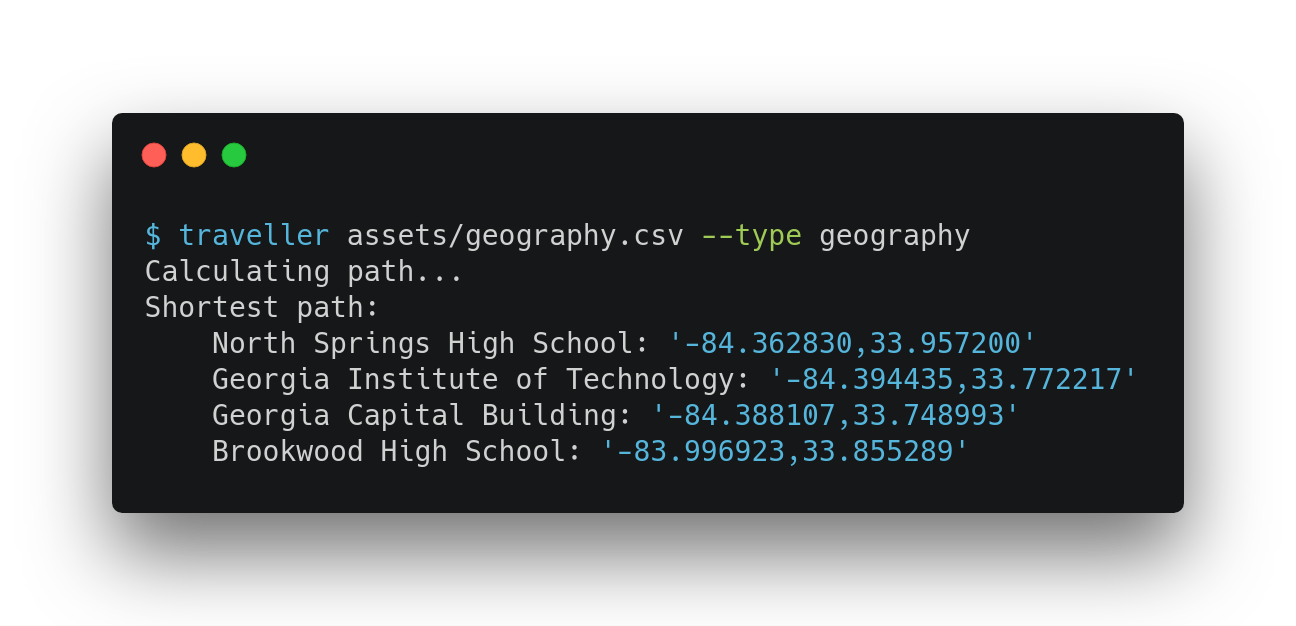
\includegraphics[width=.6\textwidth]{figures/traveller-scrot.png}
      \caption{Example usage of \texttt{Traveller}}
    \end{figure}
\end{document}
